\newpage
%%%%%%%%%%%%%%%%%%%%%%%%%%%%%%%%%%%%%%%%%%%%%%%%%%%%%%%%%%%%%%%%
%%%%%%%%%%%%%%%%%%%%%%%%%%%%%%%%%%%%%%%%%%%%%%%%%%%%%%%%%%%%%%%%
%%%%%%%%%%%%%%%%%%%%%%%%%% Enunciado %%%%%%%%%%%%%%%%%%%%%%%%%%%

\begin{myblock}
\phantomsection\addcontentsline{toc}{section}{Parte A | LSTM}
\section*{Parte A | LSTM}

    Entrena los modelos con las canciuones y con las arquitecturas RNN/LSTM/GRU. A nivel
    caracter y a nivel palabra.

\end{myblock}

%%%%%%%%%%%%%%%%%%%%%%%%%%%%%%%%%%%%%%%%%%%%%%%%%%%%%%%%%%%%%%%%
%%%%%%%%%%%%%%%%%%%%%%%%%%%%%%%%%%%%%%%%%%%%%%%%%%%%%%%%%%%%%%%%

Uno de los principales problemas de las RNN es justo lo que volvió a aquella arquitectura una herramienta tan prometedora en los inicios del NLP como lo conocemos ahora: su contexto. Recordemos que las RNN arrastran el contexto de las capas de inicio, sin importar qué tan a profundidad vaya el entrenamiento. 

De acuerdo con Dan Jurafsky, entre las razones por las cuales las RNN no logran capturar, seleccionar y llevar adelante la información más importante es que se le solicita  alos pesos y a las capas ocultas que "proporcionen información útil para la decisión actual, y actualizar y llevar hacia adelante la información requerida para decisiones futuras". 

Además, justo ir cargando con toda la información previa, y realizar la retropropagación a lo largo del tiempo, sumando la pérdida de cada capa, paso a paso, provoca lo que se conoce como "desvanecimiento del gradiente". 

La solución a este tipo de problemas acarreados por las RNN llegó tras el diseño de arquitecturas que lograban no solo mantener contexto relevante a lo largo del tiempo, sino también lograr olvidar la información no necesaria, y recordar también la información requerida para el futuro. 

\begin{figure}[h!]
    \centering
    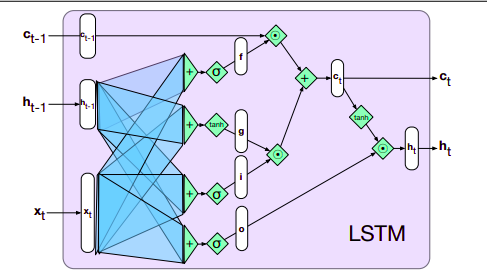
\includegraphics[width=0.8\linewidth]{Images/lstm-jurafsky.png}
    \caption{Arquitectura de una LSTM | Tomada de 'Speech Recognition' de Dan Jurafsky.}
    \label{fig:LSTM_arquitectura}
\end{figure}

Es así como se llegó a la creación de la Long Short-Term Memory (LSTM) o Red de Memoria a Largo y Corto Plazo. Este diseño no es nuevo, surgió en 1997, pero como muchas de las arquitecturas de Redes Neuronales, no fue sino hasta la década pasada que contamos con recursos suficientemente poderosos para poder entrenarlas y ponerlas en producción. 

Las LSTM realizan dos tareas principales: por un lado se encargan de eliminar información que ya no se necesita para el contexto, y por el otro lado capturan información que probablemente se utilice para la decisión siguiente. Este tipo de modelo logra aquello haciendo uso de una capa de contexto dentro de la arquitectura, además de las capas ocultas recurrentes propuestas en las RNN. Así, y mediante el uso de neuronas que utilizan compuertas para controlas el flujo de la información, logran hacer la captura del contexto relevante y no relevante. 

Dan Jurafsky lo explica de la siguiente manera: "las compuertas de una LSTM comparten un patrón de diseño común: cada una consiste en una capa de propagación hacia adelante, seguida de una función de activación sigmoide, seguida de una multiplicación elemento a elemento con la capa que se está controlando". Recordemos que la sigmoide es una función que "empuja" las salidas hacia el 0 o hacia el 1, de tal modo que al combinarla con multiplicaciones elemento a elemento, lo que estaremos logrando es poner en funcionamiento una máscara binaria que decide si los valores aprendidos en ese momento son eliminados o no. 

\subsection{Compuerta del Olvido (forget gate)}

Esta compuerta tiene como propósito eliminar información del contexto que ya es útil para la toma de decisiones futura. El proceso de eliminación es sencillo, se realiza una suma ponderada de la capa oculta del estado anterior y la entrada actual, para posteriormente pasarlo a una Sigmoide. Posteriormente, esta máscara binaria se multiplica elemento a elemento por el vector de contexto para eliminar la información que ya no es necesaria. Se define la multiplicación elemento a elemento como $\odot$, a este producto también le llamamos "producto de Hadamard". 

\[
   f_t = \sigma(U_f h_{t-1} + W_f x_t) 
\]

\[
    k_t = c_{t-1} \;\; \odot \;\; f_t 
\]

Ahora bien, para calcular la información que e va a extraer del estado oculto previo, y las 
entradas actuales, se utrilizac:

\[
  g_t = \text{tanh}(U_g h_{t-1} + W_gx_t)  
\]

\subsection{Compuerta de Adición (add gate)}

Para seleccionar la información que se agregará al contexto actual se utiliza la puerta de adición. Esta se define de la siguiente manera:

\[
    i_t = \sigma(U_i h_{t-1} + W_i x_t)
\]

\[
    j_t = g_t \;\; \odot \;\; i_t
\]

Y posteriormente sumamos esto al vector de contexto modificado para obtener nuestro nuevo vector de contexto:

\[
    c_t = j_t + k_t
\]

La compuerta de adición filtra la información nueva que está por ser añadida desde $g_t$. La diferencia clave entre la compuerta de adición y del olvido es sobre qué vector se aplican: la primera se aplica a la información nueva y la segunda se aplica al contexto previo. 

\subsection{Compuerta de Salida (output gate)}

La última compuerta en una LSTM base es la compuerta de salida. En ella se decide qué información se requiere para que el estado oculto actual. Es decir, este filtro lo que quiere hacer es tomar la decisión de que datos nos sirven para la decisión presente del modelo, no la que debe ser preservada para el futuro. Nuevamente, su estructura es similar a las anteriores:

\[
    o_t = \sigma(U_o h_{t-1} + W_o x_t)
\]

\[
    h_t = o_t \;\; \odot \;\; \text{tanh}(c_t)
\]


\subsection{Arquitectura Utilizada e Hiperparámetros}

De manera análoga al modelo GRU, se implementó y entrenó una arquitectura basada en redes de Memoria a Corto y Largo Plazo (LSTM, por sus siglas en inglés). La elección de LSTM permite una comparación directa con la arquitectura GRU, ya que ambas están diseñadas para mitigar el problema del desvanecimiento del gradiente en secuencias largas, aunque lo logran con mecanismos de compuertas (gates) ligeramente diferentes.

Nuevamente, la arquitectura se mantuvo idéntica para los entrenamientos a nivel de carácter y de palabra, con el fin de realizar una evaluación consistente.

\subsubsection{Estructura del Modelo}

El modelo LSTM se construyó con la siguiente configuración de capas:

\begin{enumerate}
    \item \textbf{Capa de Embedding:} Una capa inicial para mapear los tokens de entrada a vectores densos de 128 dimensiones.

    \item \textbf{Capas LSTM Apiladas:} El núcleo del modelo está compuesto por una pila de 6 capas LSTM, una configuración más profunda que la del modelo GRU para explorar la capacidad del modelo de aprender jerarquías de características más complejas. Cada capa cuenta con un estado oculto de 256 unidades.

    \item \textbf{Capa de Regularización (Dropout):} Se aplicó una tasa de \texttt{Dropout} del 30\% (0.3) entre las capas LSTM para prevenir el sobreajuste, una medida especialmente importante en arquitecturas más profundas.

    \item \textbf{Capa de Salida (Clasificador):} Una capa lineal final transforma la salida de la última capa LSTM al tamaño del vocabulario, empleando una activación \texttt{Softmax} para generar la distribución de probabilidad del siguiente token.
\end{enumerate}

\subsubsection{Hiperparámetros de Entrenamiento}

Los hiperparámetros de entrenamiento para el modelo LSTM se definieron como se muestra en la Tabla \ref{tab:lstm_hyperparams}. Notablemente, se utilizó un tamaño de lote mayor y un número superior de épocas en comparación con el modelo GRU para evaluar el comportamiento de la red bajo condiciones de entrenamiento más extensivas.

\begin{table}[h!]
    \centering
    \caption{Resumen de hiperparámetros de entrenamiento para el modelo LSTM.}
    \label{tab:lstm_hyperparams}
    \begin{tabular}{l|l}
        \hline
        \textbf{Hiperparámetro} & \textbf{Valor Utilizado} \\ \hline
        Optimizador & \texttt{Adam} \\
        Tasa de Aprendizaje (Learning Rate) & \texttt{5e-4 (0.0005)} \\
        Función de Pérdida & \texttt{Cross-Entropy Loss} \\
        Tamaño del Lote (Batch Size) & \texttt{64} \\
        Épocas de Entrenamiento & \texttt{15} \\ \hline
    \end{tabular}
\end{table}

\subsubsection*{PPL por época}

\begin{figure}[h!]
    \centering
    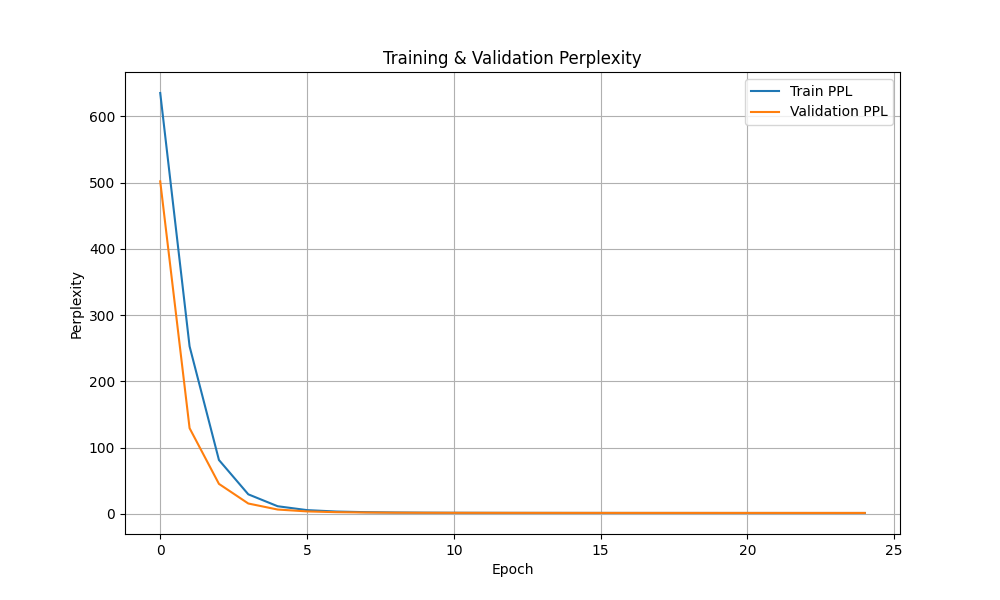
\includegraphics[width=0.7\textwidth]{Images/lstm_training_history_w.png}
    \caption{Modelo a Nivel de Palabra.}
    \label{fig:lstm_ppl_word}
\end{figure}

\subsection{Resultados}

\begin{lstlisting}[
    style=mystyle,
    caption={Output crudo del modelo LSTM a nivel de carácter.},
    label={lst:output-lstm-char}
]
I <UNK> <UNK> <UNK> <UNK> <UNK> <UNK> <UNK> s  w a y  t h a t  i t  s h o u l d  t o  l e t  t h i s  r e a t  I  d o n ' t  c a r e  w h a t ' s  i n  y o u r  h a i r  I  j u s t  w a n n a  k n o w  w h a t ' s  o n  y o u r  m i n d  I  u s e d  t o  s a y  I  w a n n a  d i e  b e f o r e  I ' m  o l d  B u t  b e c a u s e  o f  y o u ,  I  m i g h t  t h i n k  t w i c e  Y e a h ,  y e a h ,  y e a h !  Y e a h ,  y e a h ,  y e a h !  O h - o h - o h - o h - o h  Y e a h ,  y e a h ,  y e a h !  O h - o h - o h - o h - o h  Y e a h ,  y e a h ,  y e a h !  O h - o h - o h - o h - o h  Y e a h ,  y e a h ,  y e a h !  O h - o h - o h - o h - o h  Y e a h ,  y e a h ,  y e a h !  O h - o h - o h - o h - o h  Y e a h ,  y e a h ,  y e a h !  O h - o h - o h -
\end{lstlisting}

\begin{lstlisting}[
    style=mystyle,
    caption={Output crudo del modelo LSTM a nivel de palabra.},
    label={lst:output-lstm-word}
]
<UNK> like my soul but not my mind and you're living they recorded that up it) slowin' do i'm goin' all i feel some wonderin' would you be ( know you be? ) my soul 'cause is the only night, i know waging my side and the floor how my face some doors take i'm only yeah ( hates that she wrote he made in a binger and he live out if your passing gone it's another list and said my dream i'm pink, a car locomotive, and i didn't take it oh-oh-oh, they'r? asking for a second try you and i will never say it no, no, is not a little that's come up with start they're way same who-o-oa so us you've met but i am dying a friend, (ooh) home can won't you say that of a ride inspires you are not in a dream? neon waitin', wait, someone one oh, <EOS>
\end{lstlisting}

\subsection{Conclusiones}

El modelo LSTM, entrenado con un mayor número de épocas y un tamaño de lote superior al de 
GRU, mostró un desempeño robusto en términos de perplejidad. A nivel caracter, la PPL de validación
descendió de 7.75 en la primera época a valores cercanos a 1.15 en la época 12, mostrando una
notable capacidad de modelar dependencias locales en secuencias de símbolos. El output generado, 
aunque afectado por la presencia de tokens \texttt{<UNK>} de inicio, alcanzó una estructura
fonética y rítmica más clara, incluyendo patrones de repetición como ``\texttt{yeah, yeah, yeah}''. 
Si bien estos patrones son redundantes, reflejan rasgos estilísticos que no se presentaron en, por ejemplo,
el modelo de RNN. 

A nivel palabra, la PPL inicial fue muy alta, superior a los 600, pero decreció de maenra constante
hasta valores de validación cercanos a 2.24. Esto infica que el modelo aprendió a asignar probabilidades cada
vez más concentradas a secuencias posibles, aproximándose a un nivel de producción muy bueno. El texto
de output contiene frases de coherencia y con referencias reconocibles dentro del imaginario 
de la banda. Sin embargo, aún presenta estructuras fragmentadas y saltos semánticos abruptos. 

En cuanto a las métricas de novelty, el modelo LSTM alcanzó un equilibrio interesante. La 
proporción de novedad en trigramas fue de 0.92, muy cercana a la de la GRU, y superior la de la RNN.
Esto nos demuestra que, además de mantener memoria de secuencias frecuentes, la LSTM pudo recombianr
fragmentos de manera creativa, ecitando caer en mucha repetición. A nivel bigramas, se observó una tendencia
ligeramente mayor hacia la novedad con 0.65 puntos que confirman la capacida de explorar combinaciones nuevas sin
perder del todo la coherencia local. 

A nivel caracter, la PPL de este modelo es bastante bajo. A nivel palabra, la convergencia es lenta, pero
se sostiene al lograr niveles muy aceptables de PPl confirmando la utilidad del LSTM para
capturar tanto la semántica como la variedad léxica dentro de un corpus pequeño. Este modelo
supera a la RNN en cuanto a la reducción de la memorización y la maximización de la novelty. 
Sus resultados son comparables con los de la GRU, con ligera ventaja en coherencia global. 


















\clearpage




